% !TeX root = ../../../main.tex
\subsubsection{Evaluation of Textual Time Series Corpus for Sepsis}
\ChSixHeadingOnly
\paragraph{Quantitative evaluation of extracted annotations}
\label{ch06:sec:annotation_results_quantitative}
Following the quantitative evaluation protocol described in Section~\ref{ch06:sec:evaluation_methodology_metrics}, Table~\ref{ch06:tab:results} reports performance across i2m4, \texttt{sepsis-40}, and \texttt{sepsis-100}.
On the clinician-annotated \texttt{sepsis-40} set, GPT-5 is the strongest annotator across all four metrics, with event match rate 0.93, concordance 0.965, median absolute error 4 hours, and AULTC 0.822.
DeepSeek-R1 provides the next strongest overall performance on \texttt{sepsis-40}, with higher event recovery and AULTC than Llama 3.3 (event match rate 0.79 vs.\ 0.76; AULTC 0.781 vs.\ 0.742), whereas Llama 3.1 70B and Llama 3.3 show high concordance among their matched events.
This pattern highlights a recurring tradeoff in the evaluation: models can achieve high temporal ordering among the subset of events they match, while still recovering fewer reference events or producing larger absolute timestamp discrepancies.

The i2m4 results should be interpreted as a cross-schema evaluation rather than a direct in-domain test of T2S2-style extraction.
All LLM match rates are lower on i2m4, where the reference annotations are legacy i2b2-style temporal concepts rather than standalone clinical findings.
Among the LLMs, Llama 3.3 performs best on i2m4 across event match rate, concordance, median absolute error, and AULTC, and all LLMs with temporal predictions substantially outperform the BERT 5-CV time-regression baseline on AULTC.
However, the low match rates indicate that many clinically meaningful T2S2-style findings are penalized when compared against fragmented concept-level references. 
In contrast to concordances around 0.76 in i2m4, in \texttt{sepsis-40}, GPT-5 and Llama 3.3 were excellent time-ordering annotators, with concordances of 0.965 and 0.908, respectively.

On \texttt{sepsis-100}, which is a bronze-standard proxy-reference set rather than clinical ground truth, DeepSeek-R1 achieves the highest event match rate, lowest median absolute error, and highest AULTC against the GPT-5 reference, while Llama 3.3 achieves the highest concordance.
These results should therefore be read as scalable proxy-reference evaluation of extraction behavior, not as an estimate of absolute clinical accuracy.

To better understand the performance differences across datasets, we conducted an error analysis between \texttt{sepsis-10} and i2m4, presented in Appendix~\ref{ch06:apd:error-analysis}.
This analysis shows that the i2m4 performance gap is driven in part by annotation-ontology mismatch between fragmented i2b2 concepts and the more compositional clinical findings targeted by T2S2.



% !TeX root = ../../../main.tex
\begin{table}[htbp]
\caption{Comparison of event match rate (Event), median concordance ($c$), median absolute error (MAE), and area under the log-time curve (AULTC) across Llama-3.3-70B-Instruct prompt variants: no role-playing (no role), no conjunction expansion (no expansion), zero-shot, interval, and interval with i2b2 event typing (Interval + Type), for i2m4, \texttt{sepsis-40}, and \texttt{sepsis-100}.}\ChSixFloatLabel{ch06:tab:sens}
\ChSixTableBodyStart
\begin{ChSixFloatBody}

\scriptsize


\footnotesize
\centering

\begin{adjustbox}{max width=\linewidth}\begin{tabular}{l*{12}{c}}
\toprule

& \multicolumn{4}{c}{i2m4}
& \multicolumn{4}{c}{\texttt{sepsis-40}}
& \multicolumn{4}{c}{\texttt{sepsis-100}} \\

\cmidrule(lr){2-5}
\cmidrule(lr){6-9}
\cmidrule(lr){10-13}

\textbf{Model}
& \scriptsize Event
& \scriptsize c
& \scriptsize MAE
& \scriptsize AULTC
& \scriptsize Event
& \scriptsize c
& \scriptsize MAE
& \scriptsize AULTC
& \scriptsize Event
& \scriptsize c
& \scriptsize MAE
& \scriptsize AULTC \\

\midrule

L3.3 70B
& {\ChSixBfTab 0.43} & 0.768 & {\ChSixBfTab 7} & {\ChSixBfTab 0.805}
& {\ChSixBfTab 0.76} & 0.908 & 24 & 0.742
& 0.69 & 0.920 & 7 & {\ChSixBfTab 0.796} \\
\\

\textbf{Ablations} \\
No role
& 0.40 & 0.734 & 8 & 0.800
& 0.75 & 0.920 & 24 & 0.749
& 0.69 & 0.908 & 8 & 0.792 \\

No expansion
& 0.38 & 0.768 & 8 & 0.797
& 0.76 & 0.909 & 24 & {\ChSixBfTab 0.774}
& 0.69 & 0.923 & 7 & 0.795 \\

Zero-shot
& 0.30 & 0.737 & 9 & 0.794
& 0.64 & {\ChSixBfTab 0.940} & 24 & 0.746
& 0.59 & {\ChSixBfTab 0.943} & 12 & 0.786 \\
\\

\textbf{Augments} \\
Interval
& 0.43 & 0.740 & 8 & 0.798
& 0.74 & 0.924 & 24 & 0.737
& {\ChSixBfTab 0.70} & 0.902 & 10 & 0.789 \\

Interval+Type
& 0.39 & {\ChSixBfTab 0.775} & 8 & 0.803
& 0.71 & 0.911 & 28 & 0.730
& 0.68 & 0.906 & {\ChSixBfTab 6} & 0.794 \\

\bottomrule
\end{tabular}\end{adjustbox}

\end{ChSixFloatBody}
\end{table}


To examine the results in greater detail, we show figures of the cumulative distribution function of event matches and concordance boxplots (Figure \ref{ch06:fig:time-disc}) for the \texttt{sepsis-40} dataset. 
When the function reaches its maximum at the maximum cosine distance, it may be less than 1 because the label events have no events left to match, \emph{i.e.}, the reference method recovered an event that the prediction method did not. 
The event match rates in Table \ref{ch06:tab:results} correspond to the match rate at the cosine distance threshold in Figure \ref{ch06:fig:time-disc} ($\theta=0.10$).  
One could adjust the cosine distance threshold, for example, by increasing it to increase matches, at the cost of false positive matches that degrade temporal performance.
We provide a systematic threshold analysis over $\theta \in [0.01, 0.5]$ in 0.01 increments in Appendix~\ref{ch06:apd:threshold_sweep}, which demonstrates a clear elbow near $\theta=0.10$ and supports our chosen operating point.
The concordance box plots (Figure \ref{ch06:fig:time-disc}) show strong performance among the large LLMs, whereas the Llama 3.1 8B and Mixtral 8x7B model performances are much lower, which is a consistent finding throughout our analysis.

To better visualize timestamp discrepancies, we plot cumulative time-discrepancy curves among matched events (Figure~\ref{ch06:fig:time-disc}).
GPT-5 has the strongest overall time-discrepancy profile, consistent with its median absolute error of 4 hours and highest AULTC in Table~\ref{ch06:tab:results}.
The disaggregated curves further show that near-admission events are easier to timestamp than events occurring months or years away from presentation.
This degradation at longer horizons is consistent with the expert qualitative review, which identified ambiguity for events with extended duration and errors in cases requiring chained relative-time reasoning (Appendix~\ref{ch06:apd:clinician_quality_review}).
This long-horizon degradation is most visible in the bottom subpanels of Figure~\ref{ch06:fig:time-disc} (right), where the strongest models recover a larger fraction of distant events within the correct coarse time scale.

\ChSixParagraph{Sensitivity analysis of prompt components.}
The sensitivity analysis to our chosen prompt shows that prompt components affect event recovery and temporal metrics in different ways for Llama-3.3-70B-Instruct (Table~\ref{ch06:tab:sens}).
The full prompt remains a strong and balanced operating point, especially for i2m4, where it obtains the highest event match rate, lowest median absolute error, and highest AULTC.
On \texttt{sepsis-40}, removing conjunction expansion preserves the event match rate and improves AULTC, while zero-shot prompting yields higher concordance among matched events but substantially reduces event recovery.
This suggests that high concordance alone can be misleading when fewer or easier-to-order events are matched.
The interval and interval+type augmentations do not consistently improve performance: interval prompting slightly increases event match rate on \texttt{sepsis-100}, but not on \texttt{sepsis-40}, and the additional type field generally does not improve the overall balance of event recovery and temporal accuracy.
Together, these results indicate that adding output fields can increase prompt burden and does not necessarily improve the quality of the extracted textual time series across the models used.
Detailed assessments for the \texttt{sepsis-40} ablations and the i2m4 dataset, analogous to Figure~\ref{ch06:fig:time-disc}, are shown in Appendix~\ref{ch06:apd:add-perf}.



% !TeX root = ../../../main.tex
\begin{figure}[htbp]
\begin{ChSixFloatBody}

    \begin{minipage}[t]{0.24\textwidth}
    \centering
    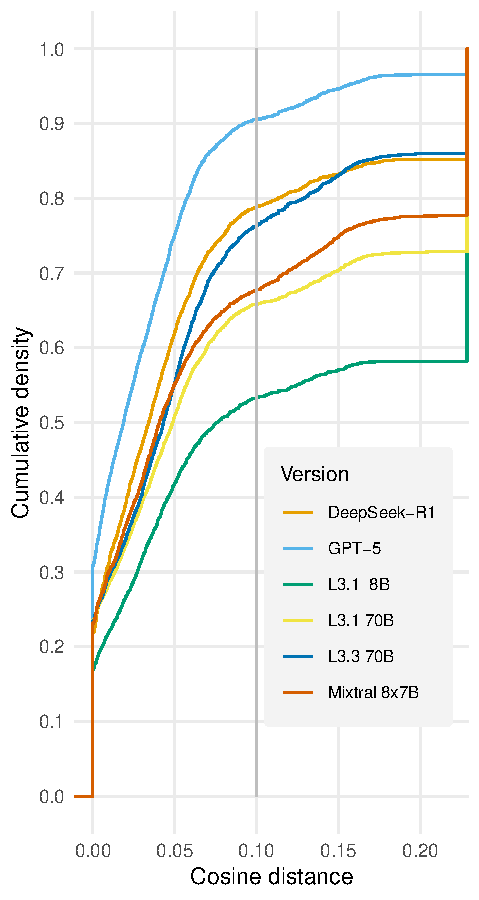
\includegraphics[width=\linewidth, page=1]{Chapters/chapter-06/images/figures/main_results_figures/figures_sepsis_40.pdf}
    \end{minipage}
    \hfill
    \begin{minipage}[t]{0.24\textwidth}
    \centering
    \includegraphics[width=\linewidth, page=2]{Chapters/chapter-06/images/figures/main_results_figures/figures_sepsis_40.pdf}
    \end{minipage}
    \begin{minipage}[t]{0.24\textwidth}
    \centering
    \includegraphics[width=\linewidth, page=3]{Chapters/chapter-06/images/figures/main_results_figures/figures_sepsis_40.pdf}
    \end{minipage}
    \begin{minipage}[t]{0.24\textwidth}
    \centering
    \includegraphics[width=\linewidth, page=4]{Chapters/chapter-06/images/figures/main_results_figures/figures_sepsis_40.pdf}
    \end{minipage}
    
    
    

\end{ChSixFloatBody}
\caption{Event match cumulative distribution function (left), concordance box-plots (middle left), 
    time discrepancy from the manual annotation timestamps among matched events, overall (middle right), and disaggregated by clinician annotator timestamp (time from presentation, right) for the \texttt{sepsis-40} dataset.}\ChSixFloatLabel{ch06:fig:time-disc}
\end{figure}


An expert qualitative review on \texttt{sepsis-10} ranked manual annotations highest, followed by O1-preview, DeepSeek-R1, and Llama 3.3; the full review protocol, ranking table, and representative error modes are provided in Appendix~\ref{ch06:apd:clinician_quality_review}.



